\begin{enumerate}[label=\thesection.\arabic*.,ref=\thesection.\theenumi]
\numberwithin{equation}{enumi}

\item The plant transfer given by
\begin{align}
G(s) = \brak{K_{P} + \frac{K_{I}}{s}}\brak{\frac{1}{s(s+2)}}
\label{eq:ee17btech11031_system1}
\end{align}
%
and shown in Figs. \ref{fig:ee17btech11031_1} and \ref{fig:ee17btech11031_2}
is known as a PI controller.

\renewcommand{\thefigure}{\theenumi.\arabic{figure}}
\begin{figure}[!ht]
	\centering
	\resizebox{\columnwidth}{!}{%\begin{figure}
\tikzstyle{block} = [draw, fill=blue!20, rectangle, 
    minimum height=1cm, minimum width=1cm]
\tikzstyle{sum} = [draw, fill=blue!20, circle, node distance=1cm]
\tikzstyle{input} = [coordinate]
\tikzstyle{output} = [coordinate]
\tikzstyle{pinstyle} = [pin edge={to-,thin,black}]

% The block diagram code is probably more verbose than necessary
\begin{tikzpicture}[auto, node distance=2cm,>=latex']
    % We start by placing the blocks
    \node [input, name=input] {};
    \node [sum, right of=input] (sum) {};
    \node [block, right of=sum] (controller) {$I = K_{I} \int e(t)$};
    \node [sum, right of=controller, node distance = 2cm] (sum2) {};
    \node [block, right of=sum2,
            node distance=2cm] (system) {Process};
    % We draw an edge between the controller and system block to 
    % calculate the coordinate u. We need it to place the measurement block. 

    \node [output, right of=system] (output) {};
    \node [block, below of=sum2] (measurements) {1};
    \node [block, above of=controller] (second){$P = K_{P} e(t)$};

    % Once the nodes are placed, connecting them is easy. 
    \draw [draw,->] (input) -- node {$r(t)$} (sum);
    \draw [->] (sum) -- node {$e(t)$} (controller);
    \draw [->] (sum) |- node[pos=0.99] {} (second);
    \draw [->] (system) -- node [name=y] {$c(t)$}(output);
    \draw [->] (controller) -- node[pos=0.99] {$+$} node[near end] {} (sum2);
    \draw [->] (second) -| node[pos=0.99] {$+$} node [near end] {} (sum2);
    \draw [->] (sum2) -- node {$u(t)$} (system);
    \draw [->] (y) |- (measurements);
    \draw [->] (measurements) -| node[pos=0.99] {$-$} node [near end] {} (sum);
\end{tikzpicture}
%\end{figure}
}
\caption{}
\label{fig:ee17btech11031_1}
\end{figure}


%
\begin{figure}[!ht]
    \centering
	\resizebox{\columnwidth}{!}{\input{./figs/ee17btech11031/ee17btech11031_tiklap.tex}}
\caption{}
\label{fig:ee17btech11031_2}
\end{figure}
\renewcommand{\thefigure}{\theenumi}

When the plant operates in a unity feedback configuration, find the condition for the stability of the closed loop system 
% \begin{enumerate}
%     \item $K_P > \frac{K_I}{2} > 0$
%     \item $2K_I > K_P > 0$
%     \item $2K_I < K_P$
%     \item $2K_I > K_P$
% \end{enumerate} 

\solution The closed Loop Transfer function for unity feedback is

\begin{align}
\frac{G\brak{s}}{\brak{1 + G(s)}} &= \frac{\brak{K_{P}s + K_{I}}}{s^2(s+2) + \brak{K_{P}s + K_{I}}}
\label{eq:ee17btech11031_system}
\\
&= \frac{(K_{P}s + K_{I})}{s^3 + 2s^2 + K_{P}s + K_{I}}
\label{eq:ee17btech11031_system}
\end{align}

Using the Routh Hurwitz tabular form
\begin{align}
\mydet{s^3\\s^2\\s^1\\s^0}
\mydet{1 & K_{P} \\ 2 & K_{I} \\ \frac{2K_{P} - K_{I}}{2} & 0 \\ K_{P}}
\end{align}

%Sufficient condition for Routh-Hurwitz Stability Criterion:- 
The sufficient condition for stability is that all the elements of the first column of the Routh array should have the same sign.
%\\
Hence, 
\begin{align}
K_{P} &> 0
\label{eq:ee17btech11031_cond1}\\
2K_{P} - K_{I} &> 0
\label{eq:ee17btech11031_cond2}\\
\implies K_{P} &> \frac{K_{I}}{2} &> 0
\label{eq:ee17btech11031_cond3}
\end{align}
%
 is the required condition for system to be stable.


\item Verify your result by plotting the gain and phase plots of \eqref{eq:ee17btech11031_system} for different values of $K_{P}$ and $K_{I}$.
\\
\solution For a system to be stable Gain Margin should be greater than 1 and Phase Margin Should be Positive.
\\
The following code plots for $K_{P} = 1$ and $K_{I} = 0.5$ Fig. \ref{fig:ee17btech11031_1}

\begin{lstlisting}
codes/ee17btech11031_1.py
\end{lstlisting}
\begin{itemize}
    \item The Phase margin: 73.07475039260186
    \item The Gain Margin: $\infty$
\end{itemize}

The Phase plot is as shown,
\begin{figure}[!ht]
  \centering
  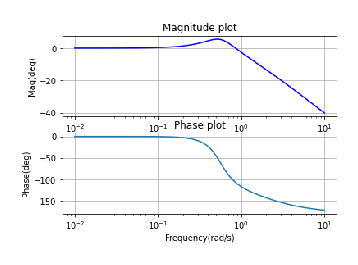
\includegraphics[width=\columnwidth]{./figs/ee17btech11031/ee17btech11031_1.eps}
  \caption{}
  \label{fig:ee17btech11031_1}
\end{figure}

For $K_{P} = -1$ and $K_{I} = 0.5$ Fig. \ref{fig:ee17btech11031_2} 

\begin{lstlisting}
codes/ee17btech11031_2.py
\end{lstlisting}
\begin{itemize}
    \item The Phase margin: -128.18015255977565
    \item The Gain Margin: $\infty$
\end{itemize}
%
The Phase plot is as shown,
\begin{figure}[!h]
  \centering
  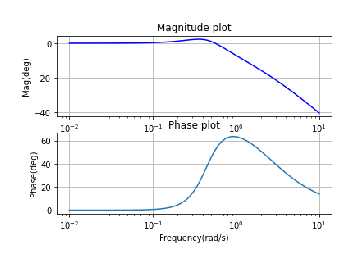
\includegraphics[width=\columnwidth]{./figs/ee17btech11031/ee17btech11031_2.eps}
  \caption{}
  \label{fig:ee17btech11031_2}
\end{figure}

%The above problem can be found in PI controller as shown:
%\begin{align}
%    u\brak{t} = K_{P} e\brak{t} + K_{I}\int e\brak{t}
%\end{align}
%Applying Laplace Transform:
%\begin{align}
%    U\brak{s} = \brak{K_{P} + \frac{K_{I}}{s}}E\brak{s}
%\end{align}
%In \eqref{eq:ee17btech11031_system1} 
%\begin{align}
%    E\brak{s} = \frac{1}{s\brak{s+2}}
%\end{align} 
\end{enumerate}
